\section{Alpine model v1 (model ID: 06)}
The Alpine model v1 model (fig.~\ref{fig:06_schematic}) is part of a top-down modelling exercise and represents a monthly water balance model \citep{Eder2003}. 
It has 2 stores and 4 parameters ($T_t$, $ddf$, $S_{max}$, $t_c$). 
The model aims to represent:

\begin{itemizecompact}
\item Snow accumulation and melt;
\item Saturation excess overland flow;
\item Linear subsurface runoff.
\end{itemizecompact}

\subsection{MARRMoT model name}
m\_06\_alpine1\_4p\_2s \\

% Equations
\subsection{Model equations}

% Model layout figure
{ 																	% This ensures it doesn't warp text further down
\begin{wrapfigure}{l}{7cm}
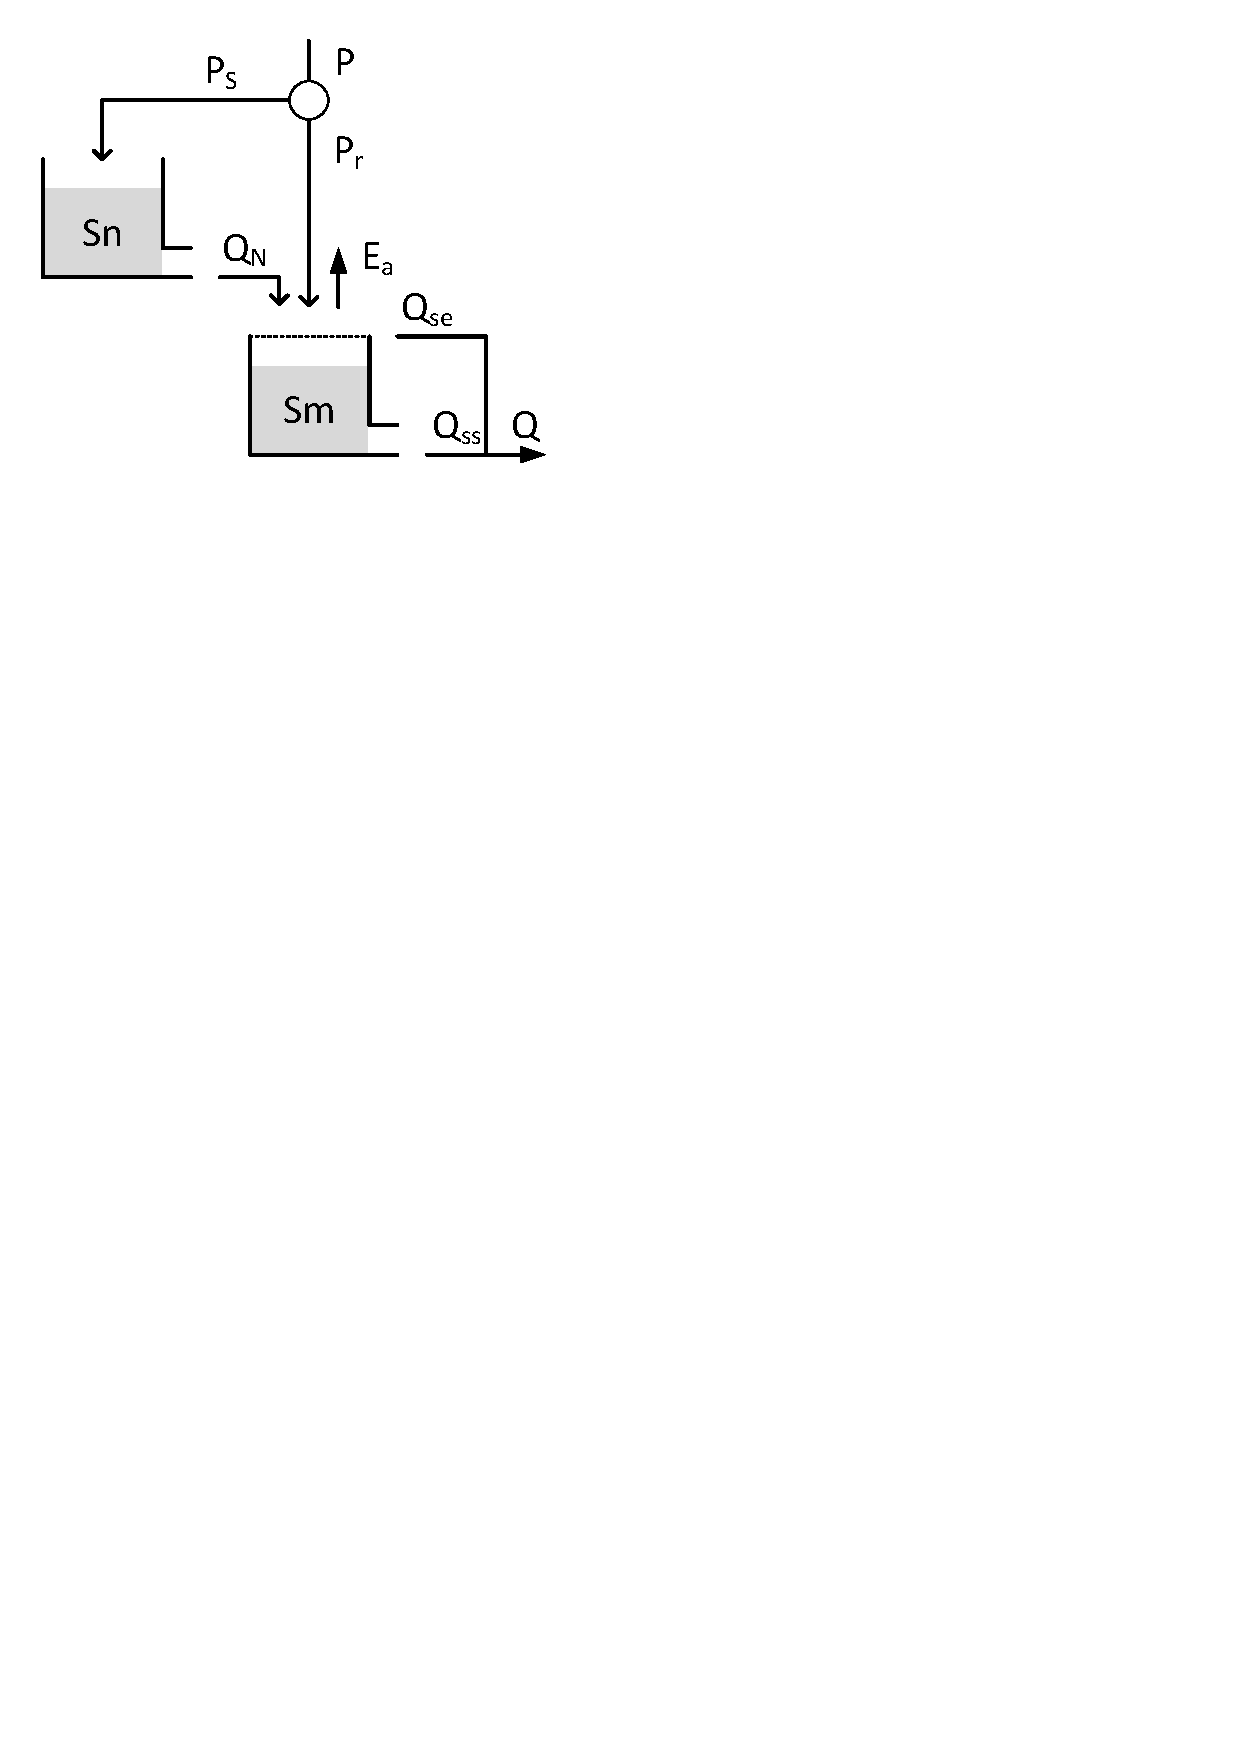
\includegraphics[trim=1cm 22cm 9cm 1cm,width=7cm,keepaspectratio]{./AppA_files/06_schematic.pdf}
\caption{Structure of the Alpine model v1} \label{fig:06_schematic}
\end{wrapfigure}

\begin{align}
	\frac{dSn}{dt} &= P_s-Q_N \\
	P_s &= \begin{cases}
		P, &\text{if } T \leq T_t \\
		0, & \text{otherwise} \\
	\end{cases} \\
	Q_N &= 
	\begin{cases}
		ddf*(T - T_t), & \text{if } T \geq T_t \\
		0, & \text{otherwise}
	\end{cases}
\end{align}

Where $S_N$ is the current snow storage [mm], $P_s$ the precipitation that falls as snow $[mm/d]$, $Q_N$ snow melt $[mm/d]$ based on a degree-day factor (ddf, [mm/\degree C/d]) and threshold temperature for snowfall and snowmelt ($T_t$, [\degree C]).

}

\begin{align}
	\frac{dS_m}{dt} &= P_r + Q_N - E_a  - Q_{se} - Q_{ss}\\
	P_r &= \begin{cases}
		P, &\text{if } T > T_t \\
		0, & \text{otherwise} \\
	\end{cases} \\
	E_a &= \begin{cases}
		E_p, &\text{if } S > 0 \\
		0, &\text{otherwise} \\
	\end{cases} \\
	Q_{se} &= \begin{cases}
		P_r + Q_N, &\text{if } S_m \geq S_{max}\\
		0, &\text{otherwise}\\
	\end{cases}\\
	Q_{ss} &= t_c*S_m	
\end{align}

Where $S_m$ [mm] is the current soil moisture storage, which is assumed to evaporate at the potential rate $E_p$ $[mm/d]$ when possible. When $S_m$ exceeds the maximum storage $S_{max}$ [mm], water leaves the model as saturation excess runoff $Q_{se}$. $Q_{ss}$ represents subsurface flow controlled by time scale parameter $t_c$ $[d^{-1}]$. Total runoff $Q_t$ $[mm/d]$ is:

\begin{equation}
	Q_t = Q_{se} + Q_{ss}
\end{equation}

\subsection{Parameter overview}
% Table generated by Excel2LaTeX from sheet 'Sheet1'
\begin{table}[htbp]
  \centering
    \begin{tabular}{lll}
    \toprule
    Parameter & Unit  & Description \\
    \midrule
    $T_t$ & $^oC$ & Threshold temperature for snowfall and melt \\
    $ddf$ & $mm~^oC^{-1}~d^{-1}$ & Degree-day factor \\
    $S_{max}$ & $mm$  & Maximum soil moisture storage \\
    $t_c$ & $d^{-1}$ & Runoff coefficient \\
    \bottomrule
    \end{tabular}%
  \label{tab:addlabel}%
\end{table}%

